\UseRawInputEncoding

%%%%%%%%%%%%%%%%%%%%%%%%%%%%%%%%%%%%%%%%%%%%%%%%%%%%%%%%%%%%%%%%%%%%%%%%%%%%%%%%
%% SETTINGS
%%%%%%%%%%%%%%%%%%%%%%%%%%%%%%%%%%%%%%%%%%%%%%%%%%%%%%%%%%%%%%%%%%%%%%%%%%%%%%%%
%% Columns
\documentclass[final,3p,times,twocolumn]{elsarticle}
%% Use the options 1p,twocolumn; 3p; 3p,twocolumn; 5p; or 5p,twocolumn
%% for a journal layout:
%% \documentclass[final,1p,times]{elsarticle}
%% \documentclass[final,1p,times,twocolumn]{elsarticle}
%% \documentclass[final,3p,times]{elsarticle}
%% \documentclass[final,3p,times,twocolumn]{elsarticle}
%% \documentclass[final,5p,times]{elsarticle}
%% \documentclass[final,5p,times,twocolumn]{elsarticle}
%% \documentclass[preprint,review,12pt]{elsarticle}

%% Image width
\newlength{\imagewidth}
\newlength{\imagescale}
%% preamble
\usepackage[english]{babel}
\usepackage[table]{xcolor} % For coloring tables
\usepackage{booktabs} % For professional quality tables
\usepackage{colortbl} % For coloring cells in tables
\usepackage{amsmath, amssymb} % For mathematical symbols and environments
\usepackage{amsthm} % For theorem-like environments
\usepackage{lipsum} % just for sample text
\usepackage{natbib}
\usepackage{graphicx}
\usepackage{indentfirst}
\usepackage{bashful}
\usepackage[margin=10pt,font=small,labelfont=bf,labelsep=endash]{caption}
\usepackage{graphicx}
\usepackage{calc}
\usepackage[T1]{fontenc} % [REVISED]
\usepackage[utf8]{inputenc} % [REVISED]
\usepackage{hyperref}
\usepackage{accsupp}
%% Line numbers
\linespread{1.1}
% \linenumbers
% Tables
\usepackage[pass]{geometry}
% \usepackage{geometry}
\usepackage{pdflscape}
\usepackage{csvsimple}
\usepackage{xltabular}
\usepackage{booktabs}
\usepackage{siunitx}
\usepackage{makecell}
\sisetup{round-mode=figures,round-precision=3}
\renewcommand\theadfont{\bfseries}
\renewcommand\theadalign{c}
\newcolumntype{C}[1]{>{\centering\arraybackslash}m{#1}}
\renewcommand{\arraystretch}{1.5}
\definecolor{lightgray}{gray}{0.95}

%% Diff
\usepackage{xcolor}
% Define commands for highlighting
% diff
\usepackage[most]{tcolorbox} % for boxes with transparency
% Define colors with transparency (opacity value)
\definecolor{GreenBG}{rgb}{0,1,0}
\definecolor{RedBG}{rgb}{1,0,0}
% Define tcolorbox environments for highlighting
\newtcbox{\greenhighlight}[1][]{%
  on line,
  colframe=GreenBG,
  colback=GreenBG!50!white, % 50% transparent green
  boxrule=0pt,
  arc=0pt,
  boxsep=0pt,
  left=1pt,
  right=1pt,
  top=2pt,
  bottom=2pt,
  tcbox raise base
}
\newtcbox{\redhighlight}[1][]{%
  on line,
  colframe=RedBG,
  colback=RedBG!50!white, % 50% transparent red
  boxrule=0pt,
  arc=0pt,
  boxsep=0pt,
  left=1pt,
  right=1pt,
  top=2pt,
  bottom=2pt,
  tcbox raise base
}
\newcommand{\REDSTARTS}{\color{red}}
\newcommand{\REDENDS}{\color{black}}
\newcommand{\GREENSTARTS}{\color{green}}
\newcommand{\GREENENDS}{\color{black}}
%%%%%%%%%%%%%%%%%%%%%%%%%%%%%%%%%%%%%%%%%%%%%%%%%%%%%%%%%%%%%%%%%%%%%%%%%%%%%%%%
%% JOURNAL NAME
%%%%%%%%%%%%%%%%%%%%%%%%%%%%%%%%%%%%%%%%%%%%%%%%%%%%%%%%%%%%%%%%%%%%%%%%%%%%%%%%
\journal{Heliyon}
%%%%%%%%%%%%%%%%%%%%%%%%%%%%%%%%%%%%%%%%%%%%%%%%%%%%%%%%%%%%%%%%%%%%%%%%%%%%%%%%
%% DOCUMENT STARTS
%%%%%%%%%%%%%%%%%%%%%%%%%%%%%%%%%%%%%%%%%%%%%%%%%%%%%%%%%%%%%%%%%%%%%%%%%%%%%%%%
\begin{document}

%%%%%%%%%%%%%%%%%%%%%%%%%%%%%%%%%%%%%%%%%%%%%%%%%%%%%%%%%%%%%%%%%%%%%%%%%%%%%%%%
%% Frontmatter
%%%%%%%%%%%%%%%%%%%%%%%%%%%%%%%%%%%%%%%%%%%%%%%%%%%%%%%%%%%%%%%%%%%%%%%%%%%%%%%%
\begin{frontmatter}
\begin{highlights}
\pdfbookmark[1]{Highlights}{highlights}

\item Neural trajectories in the hippocampus exhibited greater variability during a working memory (WM) task compared to those in the entorhinal cortex and amygdala regions.

\item The distance of neural trajectories between encoding and retrieval states in the hippocampus was memory-load dependent during a WM task.


\item Hippocampal neural trajectories fluctuated between the encoding and retrieval states in a task-dependent manner during both baseline and sharp-wave ripple (SWR) periods.

\item Hippocampal neural trajectories shifted from encoding to retrieval states during SWR period.

\end{highlights}\title{
Hippocampal neural fluctuations between memory encoding and retrieval states during a working memory task in humans
}\author[1]{Yusuke Watanabe\corref{cor1}}
\author[2,3,4]{Yuji Ikegaya}
\author[1,5]{Takufumi Yanagisawa}

\address[1]{Institute for Advanced Cocreation studies, Osaka University, 2-2 Yamadaoka, Suita, 565-0871, Osaka, Japan}
\address[2]{Graduate School of Pharmaceutical Sciences, The University of Tokyo, 7-3-1 Hongo, Tokyo, 113-0033, Japan}
\address[3]{Institute for AI and Beyond, The University of Tokyo, 7-3-1 Hongo, Tokyo, 113-0033, Japan}
\address[4]{Center for Information and Neural Networks, National Institute of Information and Communications Technology, 1-4 Yamadaoka, Suita City, 565-0871, Osaka, Japan}
\address[5]{Department of Neurosurgery, Osaka University Graduate School of Medicine, 2-2 Yamadaoka, Osaka, 565-0871, Japan}

\cortext[cor1]{Corresponding author. Tel: +81-6-6879-3652}%%Graphical abstract
%\pdfbookmark[1]{Graphical Abstract}{graphicalabstract}        
%\begin{graphicalabstract}
%\includegraphics{grabs}
%\end{graphicalabstract}
\begin{abstract}
\pdfbookmark[1]{Abstract}{abstract}
Working memory (WM) plays a vital role in many cognitive functions, though the complex neural mechanisms that support its operation are not yet fully understood. Although the importance of the hippocampus and sharp-wave ripple complexes (SWRs) -- fast, concurrent neural activities within the hippocampus -- are acknowledged in memory consolidation and retrieval, their participation in WM tasks remains somewhat ambiguous. Our study hypothesizes that multiunit activity patterns within the hippocampus cooperate synergistically with SWRs, showcasing distinctive dynamism during WM tasks. To investigate this, we carried out a thorough analysis of a dataset sourced from intracranial electroencephalogram recordings taken from the medial temporal lobe (MTL) of nine epilepsy patients performing an eight-second Sternberg task. Employing Gaussian-process factor analysis, we distinguished low-dimensional neural representations, or 'trajectories,' within the MTL regions during the WM task. Our findings showed that neural trajectories exhibited greater variation in the hippocampus compared to the entorhinal cortex and amygdala. Additionally, differences found in the trajectories between encoding and retrieval phases depended on memory load. Notably, hippocampal trajectories oscillated during the retrieval phase, demonstrating task-dependent shifts between encoding and retrieval states, along with baseline and SWR events. These oscillations transitioned from encoding to retrieval states in sync with SWRs. Consequently, our findings underscore the critical function of the hippocampus in performing WM tasks, and suggest a compelling hypothesis for further investigation: the operational state of the hippocampus shifts from encoding to retrieval during SWRs.
\end{abstract}% \pdfbookmark[1]{Keywords}{keywords}                
\begin{keyword}
working memory \sep WM \sep memory load \sep hippocampus \sep sharp-wave ripples \sep SWR \sep humans
\end{keyword}
\end{frontmatter}

%%%%%%%%%%%%%%%%%%%%%%%%%%%%%%%%%%%%%%%%%%%%%%%%%%%%%%%%%%%%%%%%%%%%%%%%%%%%%%%%
%% IMRaD
%%%%%%%%%%%%%%%%%%%%%%%%%%%%%%%%%%%%%%%%%%%%%%%%%%%%%%%%%%%%%%%%%%%%%%%%%%%%%%%%

%%%%%%%%%%%%%%%%%%%%%%%%%%%%%%%%%%%%%%%%%%%%%%%%%%%%%%%%%%%%%%%%%%%%%%%%%%%%%%%%
%% INTRODUCTION
%%%%%%%%%%%%%%%%%%%%%%%%%%%%%%%%%%%%%%%%%%%%%%%%%%%%%%%%%%%%%%%%%%%%%%%%%%%%%%%%
Working memory (WM) is vitally important in daily activities and continues to be an active research area, specifically its neural basis. The hippocampus, known to be essential for memory, consistently remains at the center of this inquiry \cite{scoville_loss_1957} \cite{squire_legacy_2009}  \cite{boran_persistent_2019} \cite{kaminski_persistently_2017} \cite{kornblith_persistent_2017} \cite{faraut_dataset_2018} \cite{borders_hippocampus_2022} \cite{li_functional_2023} \cite{dimakopoulos_information_2022}. Insights into the hippocampus's role in working memory are crucial for advancing our understanding of cognitive processes and thereby promoting developments in cognitive training and interventions.
\\
\indent
Existing evidence proposes that a temporary, synchronized oscillation, known as sharp-wave ripple (SWR) \cite{buzsaki_hippocampal_2015}, is associated with several cognitive functions, such as memory replay \cite{wilson_reactivation_1994} \cite{nadasdy_replay_1999} \cite{lee_memory_2002} \cite{diba_forward_2007} \cite{davidson_hippocampal_2009}, memory consolidation \cite{girardeau_selective_2009} \cite{ego-stengel_disruption_2010} \cite{fernandez-ruiz_long-duration_2019} \cite{kim_corticalhippocampal_2022}, memory recall \cite{wu_hippocampal_2017} \cite{norman_hippocampal_2019} \cite{norman_hippocampal_2021}, along with neural plasticity \cite{behrens_induction_2005} \cite{norimoto_hippocampal_2018}. These indications suggest that SWR might be an essential part of hippocampal processing, thus contributing to working memory performance. Yet, studies examining the effect of SWRs on working memory are limited \cite{jadhav_awake_2012}, with most research predominantly focusing on rodent models engaged in navigation tasks where the timing of memory acquisition and recall is not explicitly outlined.
\\
\indent
Recent studies have illustrated that hippocampal neurons demonstrate low-dimensional representations during WM tasks. Specifically, the firing patterns of place cells \cite{okeefe_hippocampus_1971} \cite{okeefe_place_1976} \cite{ekstrom_cellular_2003} \cite{kjelstrup_finite_2008} \cite{harvey_intracellular_2009}, located in the hippocampus, have been shown to exist within a dynamic, nonlinear three-dimensional hyperbolic geometry in rodents \cite{zhang_hippocampal_2022}. Grid cells in the entorhinal cortex (EC)—the primary pathway to the hippocampus \cite{naber_reciprocal_2001} \cite{van_strien_anatomy_2009} \cite{strange_functional_2014}—showed a toroidal topology during exploration \cite{gardner_toroidal_2022}. However, these investigations have been confined to spatial navigation tasks in rodents, thus constraining the temporal resolution of WM tasks. The implication of these findings for human subjects and their extrapolation beyond navigation tasks is yet to be confirmed.
\\
\indent
Considering these factors, this study seeks to support the hypothesis that hippocampal neurons represent low-dimensional spaces distinctively, referenced here as 'neural trajectory,' particularly during SWR periods in WM tasks. To assess this proposition, we utilized a dataset of patients executing an eight-second Sternberg task featuring high temporal resolution (1 s for fixation, 2 s for encoding, 3 s for upkeep, and 2 s for retrieval) while their intracranial electroencephalography signals (iEEG) within the medial temporal lobe (MTL) were being recorded \cite{boran_dataset_2020}. To explore low-dimensional neural trajectories, we employed Gaussian-process factor analysis (GPFA), an acclaimed strategy for analyzing neural population dynamics \cite{yu_gaussian-process_2009}.
\label{sec:introduction}
%%%%%%%%%%%%%%%%%%%%%%%%%%%%%%%%%%%%%%%%%%%%%%%%%%%%%%%%%%%%%%%%%%%%%%%%%%%%%%%%
%% METHODS
%%%%%%%%%%%%%%%%%%%%%%%%%%%%%%%%%%%%%%%%%%%%%%%%%%%%%%%%%%%%%%%%%%%%%%%%%%%%%%%%
\section{Methods}
\subsection{Dataset}
A publicly available dataset \cite{boran_dataset_2020} was used. This dataset consists of nine epilepsy patients performing a modified Sternberg task, a task incorporating four phases: fixation (1s), encoding (2s), maintenance (3s), and retrieval (2s) \cite{boran_dataset_2020}. Throughout the encoding phase, participants were introduced to four, six, or eight alphabet letters, known as the set size. These participants were then tasked to ascertain whether a probe letter, presented during the retrieval phase was previously shown (the correct choice for the Match IN task) or not (the correct choice for the Mismatch OUT task). iEEG signals were recorded at a sampling rate of 32 kHz, within a frequency range of 0.5--5,000 Hz, using depth electrodes implanted in various medial temporal lobe (MTL) regions; these include the anterior head of the left and right hippocampus (AHL and AHR), the posterior body of the hippocampus (PHL and PHR), the entorhinal cortex (ECL and ECR), and the amygdala (AL and AR), as depicted in Figure~\ref{fig:01}A and Table~\ref{tab:01}. Subsequently, these iEEG signals were downsampled to a rate of 2 kHz. Correlations among variables, such as set size and correct rate, were investigated (Figure~\ref{fig:s01}S1). The timings of multiunit spikes were determined using a spike sorting algorithm \cite{niediek_reliable_2016} via the Combinato package (\url{https://github.com/jniediek/combinato}) (Figure~\ref{fig:01}C).

\subsection{Calculation of neural trajectories using GPFA}
Neural trajectories, a.k.a. 'factors' (Figure~\ref{fig:01}D), in areas including the hippocampus, EC, and amygdala (Figure~\ref{fig:01}D), were calculated using GPFA \cite{yu_gaussian-process_2009} applied to the multiunit activity data for each session. GPFA was executed with the elephant package (\url{https://elephant.readthedocs.io/en/latest/reference/gpfa.html}). The bin size was set to 50 ms, with no overlaps. Each factor was z-normalized across all sessions. The Euclidean distance from the origin ($O$) was subsequently calculated (Figure~\ref{fig:01}E).
\\
\indent
For each trajectory within a region, e.g., AHL, \textit{geometric medians} ($\mathrm{g_{F}}$ for fixation, $\mathrm{g_{E}}$ for encoding, $\mathrm{g_{M}}$ for maintenance, and $\mathrm{g_{R}}$ for retrieval phase) were ascertained by calculating the median coordinates of the trajectory during the four phases (Figure~\ref{fig:01}D). An optimal dimensionality for GPFA was identified as three using the elbow method, derived by investigating the log-likelihood values through a three-fold cross-validation approach (Figure~\ref{fig:02}B).

\subsection{Identifying SWR candidates from hippocampal regions}
Potential SWR events within the hippocampus were detected using a widely adopted method \cite{liu_consensus_2022}. LFP signals from a specific region of interest (ROI), such as AHL, were re-referenced by subtracting an averaged signal from locations outside the ROI (\textit{e.g.}, AHR, PHL, PHR, ECL, ECR, AL, and AR) (see Figure~\ref{fig:01}A). The re-referenced LFP signals then underwent filtering with a ripple-band filter (80--140 Hz) to identify possible SWR candidates, dubbed $\textrm{SWR}^+$ candidates (see Figure~\ref{fig:01}B). SWR detection utilized a published tool (\url{https://github.com/Eden-Kramer-Lab/ripple_detection}) \cite{kay_hippocampal_2016}, with the bandpass range adjusted to 80--140 Hz for humans \cite{norman_hippocampal_2019} \cite{norman_hippocampal_2021}, deviating from the original 150--250 Hz range typically applied to rodents.
\\
\indent
Control events for $\textrm{SWR}^+$ candidates, labeled as $\textrm{SWR}^-$ candidates, were identified by randomly shuffling the timestamps of $\textrm{SWR}^+$ candidates across all trials and subjects. The resulting $\textrm{SWR}^+/\textrm{SWR}^-$ candidates were then subjected to visual inspection (Figure~\ref{fig:01}).

\subsection{Defining SWRs from putative hippocampal CA1 regions}
SWRs were distinguished from SWR candidates in presumptive CA1 regions. The regions were initially defined in the following manner: $\textrm{SWR}^+/\textrm{SWR}^-$ candidates in the hippocampus were projected into a two-dimensional space based on overlapping spike counts per unit using a supervised method called UMAP (Uniform Manifold Approximation and Projection) \cite{mcinnes_umap_2018} (Figure~\ref{fig:04}A). Clustering validation was performed by computing the silhouette score \cite{rousseeuw_silhouettes_1987} from clustered samples (Table~\ref{tab:02}). Regions in the hippocampus, which scored above 0.6 on average across sessions (75th percentile) (Figure~\ref{fig:04}B), were considered to be presumed CA1 regions, thereby identifying five electrode positions among five patients (Table~\ref{tab:03}).
\\
\indent
$\textrm{SWR}^+/\textrm{SWR}^-$ candidates in these assumed CA1 regions were reclassified as $\textrm{SWR}^+/\textrm{SWR}^-$, hence losing their candidate status. The duration and ripple band peak amplitude of SWRs were observed to conform to log-normal distributions (Figure~\ref{fig:04}4C \& E). Each time period of SWR was partitioned in relation to the time from the SWR center into pre- (at $-800$ to $-300$ ms from SWR center), mid- (at $-250$ to $+250$ ms), and post-SWR (at $+300$ to $+800$ ms) times.

\subsection{Statistical evaluation}
Statistical analyses were performed using the Brunner--Munzel and Kruskal-Wallis tests courtesy of the SciPy package in Python \cite{virtanen_scipy_2020}. The correlational analysis determined the rank of the observed correlation coefficient in its associated set-size-shuffled surrogate via a custom Python script. The bootstrap test, on the other hand, was implemented using an in-house Python script.

\label{sec:methods}
%%%%%%%%%%%%%%%%%%%%%%%%%%%%%%%%%%%%%%%%%%%%%%%%%%%%%%%%%%%%%%%%%%%%%%%%%%%%%%%%
%% RESULTS
%%%%%%%%%%%%%%%%%%%%%%%%%%%%%%%%%%%%%%%%%%%%%%%%%%%%%%%%%%%%%%%%%%%%%%%%%%%%%%%%
\section{Results}
\subsection{iEEG recording and neural trajectory in MTL regions during a Sternberg task}
We leveraged a publicly available dataset for this analysis \cite{boran_dataset_2020}. This dataset encompasses LFP signals (Figure 1A) from MTL regions (Table~\ref{tab:01}) during a modified Sternberg task execution. We identified SWR$^+$ candidates from LFP signals filtered through the 80--140 Hz ripple band (Figure 1B), originating across all hippocampal regions (refer to Methods). Correspondingly, SWR$^-$ candidates were defined at identical timestamps) but shuffled across different trials (Figure 1). The dataset included multiunit spikes (Figure 1C) identified via a spike sorting algorithm \cite{niediek_reliable_2016}. By employing GPFA \cite{yu_gaussian-process_2009}, and using the 50-ms binned multiunit activity with no overlaps, we determined the neural trajectories (or factors) of MTL regions by session and region (Figure 1D). We normalized each factor by session and region for instance, session \#2 in AHL of subject \#1. Subsequently, we calculated the Euclidean distance from the origin ($O$) (Figure 1E).

\subsection{Hippocampal neural trajectory correlation with a Sternberg task}
Figure 2A illustrates the cloud of median neural trajectories of 50 trials within the three main factor spaces. We determined the optimal embedding dimension for the GPFA model to be three, using the elbow method (Figure 2B). The trajectory distance from the origin ($O$) (represented as $\mathrm{\lVert g_{F} \rVert}$, $\mathrm{\lVert g_{E} \rVert}$, $\mathrm{\lVert g_{M} \rVert}$, and $\mathrm{\lVert g_{R} \rVert}$) in the hippocampus exceeded corresponding distances in the EC and amygdala (Figures 2C and D).\footnote{Hippocampus: Distance = 1.11 [1.01], median [IQR], \textit{n} = 195,681 timepoints; EC: Distance = 0.94 [1.10], median [IQR], \textit{n} = 133,761 timepoints; Amygdala: Distance = 0.78 [0.88], median [IQR], \textit{n} = 165,281 timepoints.}
\\
\indent
Similarly, we computed the distances between the geometric medians of four phases, namely $\mathrm{\lVert g_{F}g_{E} \rVert}$, $\mathrm{\lVert g_{F}g_{M} \rVert}$, $\mathrm{\lVert g_{F}g_{R} \rVert}$, $\mathrm{\lVert g_{E}g_{M} \rVert}$, $\mathrm{\lVert g_{E}g_{R} \rVert}$, and $\mathrm{\lVert g_{M}g_{R} \rVert}$. The results indicated that the hippocampus displayed larger distances between phases than both the EC and amygdala. \footnote{Hippocampus: Distance = 0.60 [0.70], median [IQR], \textit{n} = 8,772 combinations; EC: Distance = 0.28 [0.52], median [IQR], \textit{n} = 5,017 combinations (\textit{p} $<$ 0.01; Brunner--Munzel test); Amygdala: Distance = 0.24 [0.42], median [IQR], \textit{n} = 7,466 combinations (\textit{p} $<$ 0.01; Brunner--Munzel test).}

\subsection{Memory load-dependent neural trajectory distance between encoding and retrieval states in the hippocampus}
In terms of memory load in the Stenberg task, we identified a negative correlation between the correct rate of trials and set size (the number of letters to encode) (Figure 3A).\footnote{Correct rate: set size four (0.99 \textpm 0.11, mean \textpm SD; \textit{n} = 333 trials) vs. set size six (0.93 \textpm 0.26; \textit{n} = 278 trials; \textit{p} $<$ 0.001, Brunner--Munzel test with Bonferroni correction) and set size eight (0.87 \textpm 0.34; \textit{n} = 275 trials; \textit{p} $<$ 0.05; Brunner--Munzel test with Bonferroni correction). Overall, \textit{p} $<$ 0.001 for Kruskal--Wallis test; correlation coefficient = - 0.20, \textit{p} $<$ 0.001.} Similarly, a positive correlation was observed between the response time and set size (Figure 3B).\footnote{Response time: set size four (1.26 \textpm 0.45 s; \textit{n} = 333 trials) vs. set size six (1.53 \textpm 0.91 s; \textit{n} = 278 trials) and set size eight (1.66 \textpm 0.80 s; \textit{n} = 275 trials). All comparisons \textit{p} $<$ 0.001, Brunner--Munzel test with Bonferroni correction; \textit{p} $<$ 0.001 for Kruskal--Wallis test; correlation coefficient = 0.22, \textit{p} $<$ 0.001}.
\\
\indent
Furthermore, we found a positive correlation between set size and the trajectory distance between the encoding and retrieval phases ($\mathrm{log_{10}\lVert g_{E}g_{R} \rVert}$) (Figure 3C).\footnote{Correlation between set size and $\mathrm{log_{10}(\lVert g_{E}g_{R} \rVert}$): correlation coefficient = 0.05, \textit{p} $<$ 0.001. Specific values: $\mathrm{\lVert g_{E}g_{R} \rVert}$ = 0.54 [0.70] for set size four, \textit{n} = 447; $\mathrm{\lVert g_{E}g_{R} \rVert}$ = 0.58 [0.66] for set size six, \textit{n} = 381; $\mathrm{\lVert g_{E}g_{R} \rVert}$ = 0.61 [0.63] for set size eight, \textit{n} = 395.}. However, distances between other combinations of phases did not display statistically significant correlations (Figures 3D and S2).

\subsection{Detection of hippocampal SWR from putative CA1 regions}
For precision improvement in recording sites and SWR detection, we estimated the electrode placements in the CA1 regions of the hippocampus using distinct multiunit spike patterns during the SWR events. SWR$^+$/SWR$^-$ candidates from every session and hippocampal region were embedded in a two-dimensional space using UMAP (Figure 4A).\footnote{Consider the AHL in session \#1 of subject \#1, for illustration purposes.} We used the silhouette score as a metric for quality of clustering (Figure 4B and Table~\ref{tab:02}). Recording sites with an average silhouette score exceeding 0.6 across all sessions were identified as putative CA1 regions.\footnote{The identified regions were: AHL of subject \#1, AHR of subject \#3, PHL of subject \#4, AHL of subject \#6, and AHR of subject \#9.} (Tables~\ref{tab:02} and \ref{tab:03}). We identified five putative CA1 regions, four of which were not labeled as seizure onset zones (Table~\ref{tab:01}).
\\
\indent
Subsequently, SWR$^+$/SWR$^-$ candidates within these putative CA1 regions were labeled as SWR$^+$ and SWR$^-$, respectively\footnote{These definitions led to equal counts for both categories: SWR$^+$ (\textit{n} = 1,170) and SWR$^-$ (\textit{n} = 1,170).}  (Table~\ref{tab:03}). Both SWR$^+$ and SWR$^-$ exhibited the same duration\footnote{These definitions led to equal durations for both categories: SWR$^+$ (93.0 [65.4] ms) and SWR$^-$ (93.0 [65.4] ms).}  (Figure 4C) due to their definitions, and followed a log-distribution. We observed an augmentation in SWR$^+$ incidence during the initial 400 ms of the retrieval phase\footnote{SWR$^+$ increased against the bootstrap sample; 95th percentile = 0.42 [Hz]; \textit{p} $<$ 0.05.}  (Figure 4D). The peak ripple band amplitude of SWR$^+$ outpaced SWR$^-$ and followed a log-normal distribution (Figure 4E).\footnote{SWR$^+$ (3.05 [0.85] SD of baseline, median [IQR]; \textit{n} = 1,170) vs. SWR$^-$ (2.37 [0.33] SD of baseline, median [IQR]; \textit{n} = 1,170; \textit{p} $<$ 0.001; Brunner--Munzel test).}.

\subsection{Transient changes in hippocampal neural trajectory during SWR}
We computed the distance of the trajectory from the origin ($O$) during SWR events in both the encoding and retrieval phases (Figure 5A). Observing the increase in distance during SWR as shown in Figure 5A, we differentiated each SWR into three stages: pre-, mid-, and post-SWR. Therefore, the distances from $O$ during those SWR periods are identified as $\mathrm{\lVert \text{pre-eSWR}^+ \rVert}$, $\mathrm{\lVert \text{mid-eSWR}^+ \rVert}$ among others.
\\
\indent
$\mathrm{\lVert \text{mid-eSWR}^+ \rVert}$\footnote{1.25 [1.30], median [IQR], \textit{n} = 1,281, in Match IN task; 1.12 [1.35], median [IQR], \textit{n} = 1,163, in Mismatch OUT task} was greater than $\mathrm{\lVert \text{pre-eSWR}^+ \rVert}$\footnote{1.08 [1.07], median [IQR], \textit{n} = 1,149, in Match IN task; 0.90 [1.12], median [IQR], \textit{n} = 1,088, in Mismatch OUT task}, and $\mathrm{\lVert \text{mid-rSWR}^+ \rVert}$\footnote{1.32 [1.24], median [IQR], \textit{n} = 935, in Match IN task; 1.15 [1.26], median [IQR], \textit{n} = 891, in Mismatch OUT task} was larger than $\mathrm{\lVert \text{pre-rSWR}^+ \rVert}$ in both Match IN and Mismatch OUT tasks.\footnote{1.19 [0.96], median [IQR], \textit{n} = 673, in Match IN task; 0.94 [0.88], median [IQR], \textit{n} = 664, in Mismatch OUT task}.

\subsection{Visualization of hippocampal neural trajectory during SWR in two-dimensional spaces}
Following our observations of neural trajectory 'jumping' during SWR (Figure 5), we visualized the three-dimensional trajectories of pre-, mid-, and post-SWR events during the encoding and retrieval phases (Figure 6), the distance between which was found to be memory-load dependent (Figure 3).
\\
\indent
To provide two-dimensional visualization, we linearly aligned peri-SWR trajectories by assigning $\mathrm{g_{E}}$ at the origin (0, 0) and $\mathrm{g_{R}}$ at ($\mathrm{\lVert g_{E}g_{R} \rVert}$, 0). Post this, we rotated these aligned trajectories around the $\mathrm{g_{E}g_{R}}$ axis (the x-axis). Thus, the distances from the origin in the original three-dimensional spaces are preserved in the two-dimensional equivalent.
\\
\indent
The scatter plot within these two-dimensional spaces reveals characteristic distributions of peri-SWR trajectories based on phases and task types. For instance, one can observe that the magnitude of  $\mathrm{\lVert \text{mid-eSWR}^+ \rVert}$ surpasses that of $\mathrm{\lVert \text{pre-eSWR}^+ \rVert}$ (Figure 6B), consistent with our earlier findings (Figure 5).

\subsection{Fluctuations of hippocampal neural trajectories between encoding and retrieval states}
Next, we examined trajectory \textit{directions} in relation to $\overrightarrow{\mathrm{g_{E}g_{R}}}$. The directions of SWRs were defined by the neural trajectory at $-250$ ms and $+250$ ms from their center, i.e., $\overrightarrow{\mathrm{eSWR^+}}$.
\\
\indent
We calculated the density of $\overrightarrow{\mathrm{eSWR}} \cdot \overrightarrow{\mathrm{g_{E}g_{R}}}$, $\overrightarrow{\mathrm{rSWR}} \cdot \overrightarrow{\mathrm{g_{E}g_{R}}}$, and $\overrightarrow{\mathrm{eSWR}} \cdot \overrightarrow{\mathrm{rSWR}}$ (Figures 7A--D). $\overrightarrow{\mathrm{rSWR^-}} \cdot \overrightarrow{\mathrm{g_{E}g_{R}}}$ displayed a biphasic distribution.
\\
\indent
By taking the difference between the distribution of $\overrightarrow{\mathrm{rSWR^+}} \cdot \overrightarrow{\mathrm{g_{E}g_{R}}}$ (Figures 7A and B) and that of $\overrightarrow{\mathrm{rSWR^-}} \cdot \overrightarrow{\mathrm{g_{E}g_{R}}}$ (Figures 7C and D), we computed the contributions of SWR (Figures 7E and F), which revealed a shift in the direction of $\overrightarrow{\mathrm{g_{E}g_{R}}}$ (Figures 7E and F: \textit{red rectangles}).
\\
\indent
Moreover, exclusively in the Mismatch OUT task, $\overrightarrow{\mathrm{eSWR^+}} \cdot \overrightarrow{\mathrm{rSWR^+}}$ was less than $\overrightarrow{\mathrm{eSWR^-}} \cdot \overrightarrow{\mathrm{rSWR^-}}$ (baseline periods) (Figure 7F: \textit{pink circles}). In simpler terms, eSWR and rSWR pointed in the opposite direction only in the Mismatch OUT task but not in the Match IN task (Figure 7E: \textit{pink circles}).
\label{sec:results}\section{Discussion}
%%%%%%%%%%%%%%%%%%%%%%%%%%%%%%%%%%%%%%%%%%%%%%%%%%%%%%%%%%%%%%%%%%%%%%%%%%%%%%%%
%% DISCUSSION
%%%%%%%%%%%%%%%%%%%%%%%%%%%%%%%%%%%%%%%%%%%%%%%%%%%%%%%%%%%%%%%%%%%%%%%%%%%%%%%%
\section{Discussion}
This study proposed that within low-dimensional spaces during a working memory (WM) task in humans, hippocampal neurons shape unique trajectories, especially during sharp-wave ripple (SWR) periods. Initially, we projected the multiunit spikes from medial temporal lobe (MTL) regions onto three-dimensional spaces during a Sternberg task using Gaussian Process Factor Analysis (GPFA) (Figure~\ref{fig:01}D--E and Figure~\ref{fig:02}A). We noted that the trajectory distance across WM phases ($\mathrm{\lVert g_{F}g_{E} \rVert}$, $\mathrm{\lVert g_{F}g_{M} \rVert}$, $\mathrm{\lVert g_{F}g_{R} \rVert}$, $\mathrm{\lVert g_{E}g_{M} \rVert}$, $\mathrm{\lVert g_{E}g_{R} \rVert}$, and $\mathrm{\lVert g_{M}g_{R} \rVert}$) was significantly larger in the hippocampus than in the entorhinal cortex (EC) and amygdala (Figure~\ref{fig:02}E). This revelation indicated dynamic neural activity in the hippocampus during the WM task. Furthermore, a positive correlation between the trajectory distance from the encoding to the retrieval phase ($\mathrm{\lVert g_{F}g_{E} \rVert}$) and memory load was seen in the hippocampus (Figure~\ref{fig:03}C--D), which reflected WM processing. Transient increases were discovered in the hippocampal neural trajectory during SWRs (Figure~\ref{fig:05}). Lastly, the hippocampal neural trajectory switched between encoding and retrieval states, transitioning from encoding to retrieval during SWR events (Figure~\ref{fig:07}). These findings not only elucidate varying aspects of hippocampal neural activity during a WM task in humans but also offer new insights into how SWRs influence the switch in neural states.

The distance of the neural trajectory across the phases was discovered to be greater in the hippocampus compared to that in the EC and amygdala, even when considering the distance from $O$ in these regions (Figure~\ref{fig:02}C--E). This evidence backs the involvement of the hippocampus in the WM task, in agreement with prior reports of persistent firing within the hippocampus during the maintenance phase \cite{boran_persistent_2019} \cite{kaminski_persistently_2017} \cite{kornblith_persistent_2017} \cite{faraut_dataset_2018}. However, when GPFA was applied to multiunit activity at 1-second-level resolution during the WM task, the neural trajectory in low-dimensional space displayed a memory load dependence between the encoding and retrieval phases, expressed as $\mathrm{\lVert g_{E}g_{R} \rVert}$ (Figure~\ref{fig:03}). This result reinforces the association between the hippocampus and WM processing.

The analysis concentrated on putative CA1 regions (Figure~\ref{fig:04}), corroborated by multiple factors. This specific focus originates from established observations that SWRs synchronize with spike bursts of interneurons and pyramidal neurons \cite{buzsaki_two-stage_1989} \cite{quyen_cell_2008} \cite{royer_control_2012} \cite{hajos_input-output_2013}, potentially within a 50 $\mu$m radius of the recording site \cite{schomburg_spiking_2012}. We also noticed a heightened incidence of SWRs during the first 0--400 ms of the retrieval phase (Figure~\ref{fig:04}D), which is consistent with previous findings of increased SWR occurrence preceding spontaneous verbal recall \cite{norman_hippocampal_2019} \cite{norman_hippocampal_2021}, reinforcing our results under a triggered retrieval condition. The observed log-normal distributions of both SWR duration and ripple band peak amplitude in this research (Figure~\ref{fig:04}C \& E) conform to the consensus in this field \cite{liu_consensus_2022}. Consequently, limiting recording sites to putative CA1 regions likely improved the accuracy of SWR detection. However, the increase in trajectory distance from $O$ during SWRs (Figure~\ref{fig:05}) may have been biased towards higher values due to channel selection. Nevertheless, this potential bias does not significantly challenge our main findings.

Interestingly, trajectory directions oscillated between encoding and retrieval states during both baseline and SWR periods in the retrieval phase (Figure~\ref{fig:07}C \& D). Moreover, the balance of this oscillation switched from the encoding state to the retrieval state during SWR events (Figure~\ref{fig:07} E \& F). These results align with previous reports on the role of SWR in memory retrieval \cite{norman_hippocampal_2019} \cite{norman_hippocampal_2021}. Our findings shed a new light, suggesting that SWRs occur when the hippocampal representation transitions from encoding to retrieval states. Thus, these findings unmask two novel aspects of hippocampal representations: (i) neuronal oscillation between encoding and retrieval states during a WM task and (ii) SWR acting as a trigger for shifting neural states.

Additionally, our study unveiled WM-task type-specific differences between encoding- and retrieval-SWRs (Figure~\ref{fig:07}E--F). Importantly, opposing movements of encoding-SWR (eSWR) and retrieval-SWR (rSWR) were not demonstrated in the Match IN task but were clear in the Mismatch OUT task. These results can be explained by memory engram theory \cite{liu_optogenetic_2012}, which posits that the Match In task provided participants with previously presented letters, whereas the Mismatch OUT task introduced a new letter not present in the encoding phase. These interpretations underline the significant role of SWR in human cognitive processes.

In conclusion, this investigation demonstrated that hippocampal activity oscillates between encoding and retrieval states during a WM task and uniquely transitions from encoding to retrieval during SWR events. These findings offer substantial insight into the neural mechanisms and functionality of working memory in the hippocampus.
\label{sec:discussion}


%%%%%%%%%%%%%%%%%%%%%%%%%%%%%%%%%%%%%%%%%%%%%%%%%%%%%%%%%%%%%%%%%%%%%%%%%%%%%%%%
%% REFERENCE STYLES
%%%%%%%%%%%%%%%%%%%%%%%%%%%%%%%%%%%%%%%%%%%%%%%%%%%%%%%%%%%%%%%%%%%%%%%%%%%%%%%%
\pdfbookmark[1]{References}{references}
\bibliography{bibliography}
% Note Re-compile is required

%% Numbering Style (sorted)
\bibliographystyle{elsarticle-num}

% Author Style
% \bibliographystyle{plainnat}
% use \citet{}

%% Numbering Style (not-sorted) 
% \bibliographystyle{plainnat}
% use \cite{}



%%%%%%%%%%%%%%%%%%%%%%%%%%%%%%%%%%%%%%%%%%%%%%%%%%%%%%%%%%%%%%%%%%%%%%%%%%%%%%%%
%% ADDITIONAL INFORMATION
%%%%%%%%%%%%%%%%%%%%%%%%%%%%%%%%%%%%%%%%%%%%%%%%%%%%%%%%%%%%%%%%%%%%%%%%%%%%%%%%
\pdfbookmark[1]{Additional Information}{additional_information}

\pdfbookmark[2]{Contributors}{contributors}                    
\section*{Contributors}
Y.W. and T.Y. conceptualized the study; Y.W. performed the data analysis; Y.W. and T.Y. wrote the original draft; and all authors reviewed the final manuscript.
\label{contributors}

\pdfbookmark[2]{Acknowledgments}{acknowledgments}                    
\section*{Acknowledgments}
This research was funded by a grant from the Exploratory Research for Advanced Technology (JPMJER1801).
\label{acknowledgments}

\pdfbookmark[2]{Declaration of Interests}{declaration_of_interest}                    
\section*{Declaration of Interests}
The authors declare that they have no competing interests.
\label{declaration of interests}

\pdfbookmark[2]{Data and code availability}{data_and_code_availability}                    
\section*{Data and code availability}
The data is available on G-Node (\url{https://doi.gin.g-node.org/10.12751/g-node.d76994/}). The source code is available on GitHub (\url{https://github.com/yanagisawa-lab/hippocampal-neural-fluctuation-during-a-WM-task-in-humans}).
\label{data and code availability}

\pdfbookmark[2]{Inclusion and Diversity Statement}{inclusion_and_diversity_statement}        
\section*{Inclusion and Diversity Statement}
We support inclusive, diverse, and equitable conduct of research.
\label{inclusion and diversity statement}

\pdfbookmark[2]{Declaration of Generative AI in Scientific Writing}{declaration_of_generative_ai}
\section*{Declaration of Generative AI in Scientific Writing}
The authors employed ChatGPT, provided by OpenAI, for enhancing the manuscript's English language quality. After incorporating the suggested improvements, the authors meticulously revised the content. Ultimate responsibility for the final content of this publication rests entirely with the authors.
\label{declaration of generative ai in scientific writing}

%% \pdfbookmark[2]{Appendices}{appendices}                    
%% \appendix
%% \section{}
%% \label{}

%%%%%%%%%%%%%%%%%%%%%%%%%%%%%%%%%%%%%%%%%%%%%%%%%%%%%%%%%%%%%%%%%%%%%%%%%%%%%%%%
%% TABLES
%%%%%%%%%%%%%%%%%%%%%%%%%%%%%%%%%%%%%%%%%%%%%%%%%%%%%%%%%%%%%%%%%%%%%%%%%%%%%%%%
\clearpage
\section*{Tables}
\label{tables}
\pdfbookmark[1]{Tables}{tables}
\pdfbookmark[2]{ID 01}{id_01}
\begin{table*}[htbp]
\centering
\small
\begin{tabular}{*{11}{c}}
\toprule
\textbf{\thead{Subject ID}} &\textbf{\thead{# of sessions}} &\textbf{\thead{AHL}} &\textbf{\thead{AHR}} &\textbf{\thead{PHL}} &\textbf{\thead{PHR}} &\textbf{\thead{ECL}} &\textbf{\thead{ECR}} &\textbf{\thead{AL}} &\textbf{\thead{AR}} &\textbf{\thead{SOZ
}} &\\
\midrule
#1 & 4 & o & x & o & o & o & x & o & x & "AHR, LR" & 
\\
\rowcolor{lightgray}
#2 & 7 & o & o & o & o & o & o & o & o & "AHR, PHR" & 
\\
#3 & 3 & o & o & o & o & o & o & o & x & "AHL, PHL" & 
\\
\rowcolor{lightgray}
#4 & 2 & o & o & o & o & o & o & o & o & "AHL, AHR, PHL, PHR" & 
\\
#5 & 3 & o & x & x & o & x & x & o & x & DRR
\\
\rowcolor{lightgray}
#6 & 6 & o & o & o & o & o & o & o & o & "AHL, PHL, ECL, AL" & 
\\
#7 & 4 & o & o & o & o & o & o & o & o & "AHR, PHR" & 
\\
\rowcolor{lightgray}
#8 & 5 & o & o & o & o & o & o & o & o & ECR
\\
#9 & 2 & o & o & o & o & o & o & o & o & "ECR, AR" & 
\\
\bottomrule
\end{tabular}
\captionsetup{width=\textwidth}
\captionsetup{width=1\textwidth}
\caption{\textbf{
Distribution of Electrodes within the Dataset
}
\smallskip
\\
This figure depicts the locations of the electrodes as well as the seizure onset zones. The regions marked by an "o" denote their inclusion in the dataset, while those identified by an "x" (\textit{in navy}) are absent. The abbreviations used are: AHL, left hippocampal head; AHR, right hippocampal head; PHL, left hippocampal body; PHR, right hippocampal body; ECL, left entorhinal cortex; ECR, right entorhinal cortex; AL, left amygdala; AR, right amygdala; and SOZ, which stands for seizure onset zone.
}
% width=1\textwidth
\label{tab:01}
\end{table*}
\restoregeometry
\pdfbookmark[2]{ID 02}{id_02}
\begin{table*}[htbp]
\centering
\small
\begin{tabular}{*{5}{c}}
\toprule
\textbf{\thead{Subject}} &\textbf{\thead{AHL}} &\textbf{\thead{AHR}} &\textbf{\thead{PHL}} &\textbf{\thead{PHR
}} &\\
\midrule
#1 & 0.60 ± 0.14 & n.a. & n.a. & 0.1 ± 0
\\
\rowcolor{lightgray}
#2 & 0.21 ± 0.16 & 0.17 ± 0.21 & 0.18 ± 0.22 & 0.20 ± 0.15
\\
#3 & 0.40 ± 0.42 & 0.83 ± 0.12 & n.a. & n.a.
\\
\rowcolor{lightgray}
#4 & 0.10 ± 0.00 & 0.10 ± 0.00 & 0.90 ± 0.00 & 0.10 ± 0.14
\\
#5 & n.a. & n.a. & n.a. & n.a.
\\
\rowcolor{lightgray}
#6 & 0.63 ± 0.06 & n.a. & n.a. & 0.27 ± 0.06
\\
#7 & 0.10 ± 0.00 & 0.35 ± 0.35 & 0.37 ± 0.47 & 0.10 ± 0.00
\\
\rowcolor{lightgray}
#8 & 0.13 ± 0.10 & n.a. & 0.28 ± 0.49 & n.a.
\\
#9 & n.a. & 0.85 ± 0.07 & 0.15 ± 0.07 & n.a.
\\
\bottomrule
\end{tabular}
\captionsetup{width=\textwidth}
\caption{\textbf{
Silhouette score of UMAP clustering for $SWR^+$ candidates and $SWR^-$ candidates
}
\smallskip
\\
The silhouette scores (mean ± SD across sessions per subject) for UMAP clustering of SWR+ candidates and SWR− candidates were computed from the corresponding multiunit spike patterns. The mean values were 0.205, with a standard deviation of 0.285, and median [IQR]; (Figure 4A and 4B).
}
% width=1\textwidth
\label{tab:02}
\end{table*}
\restoregeometry
\pdfbookmark[2]{ID 03}{id_03}
\begin{table*}[htbp]
\centering
\small
\begin{tabular}{*{6}{c}}
\toprule
\textbf{\thead{Subject ID}} &\textbf{\thead{# of sessions}} &\textbf{\thead{# of trials}} &\textbf{\thead{ROI}} &\textbf{\thead{# of SWRs}} &\textbf{\thead{SWR incidence [Hz]
}} &\\
\midrule
#1 & 2 & 100 & AHL & 274 & 0.34
\\
\rowcolor{lightgray}
#3 & 2 & 97 & AHR & 325 & 0.42
\\
#4 & 2 & 99 & PHL & 202 & 0.26
\\
\rowcolor{lightgray}
#6 & 2 & 100 & AHL & 297 & 0.37
\\
#9 & 2 & 97 & AHR & 72 & 0.09
\\
\rowcolor{lightgray}
Total = 10 & Total = 493 & "Total = 1,170" & 0.30 ± 0.13 (mean ± SD)
\\
\bottomrule
\end{tabular}
\captionsetup{width=\textwidth}
\caption{\textbf{
Accounting for Specified SWR Events
}
\smallskip
\\
The table collects statistics pertaining to the putative CA1 regions and SWR events. To minimize sampling bias, only the first two sessions (sessions #1 and #2) from each subject were taken into consideration.
}
% width=1\textwidth
\label{tab:03}
\end{table*}
\restoregeometry

%%%%%%%%%%%%%%%%%%%%%%%%%%%%%%%%%%%%%%%%%%%%%%%%%%%%%%%%%%%%%%%%%%%%%%%%%%%%%%%%
%% FIGURES
%%%%%%%%%%%%%%%%%%%%%%%%%%%%%%%%%%%%%%%%%%%%%%%%%%%%%%%%%%%%%%%%%%%%%%%%%%%%%%%%
\clearpage
\section*{Figures}
\label{figures}
\pdfbookmark[1]{Figures}{figures}
        \clearpage
        \begin{figure*}[ht]
            \pdfbookmark[2]{ID 01}{figure_id_01}
        	\centering
            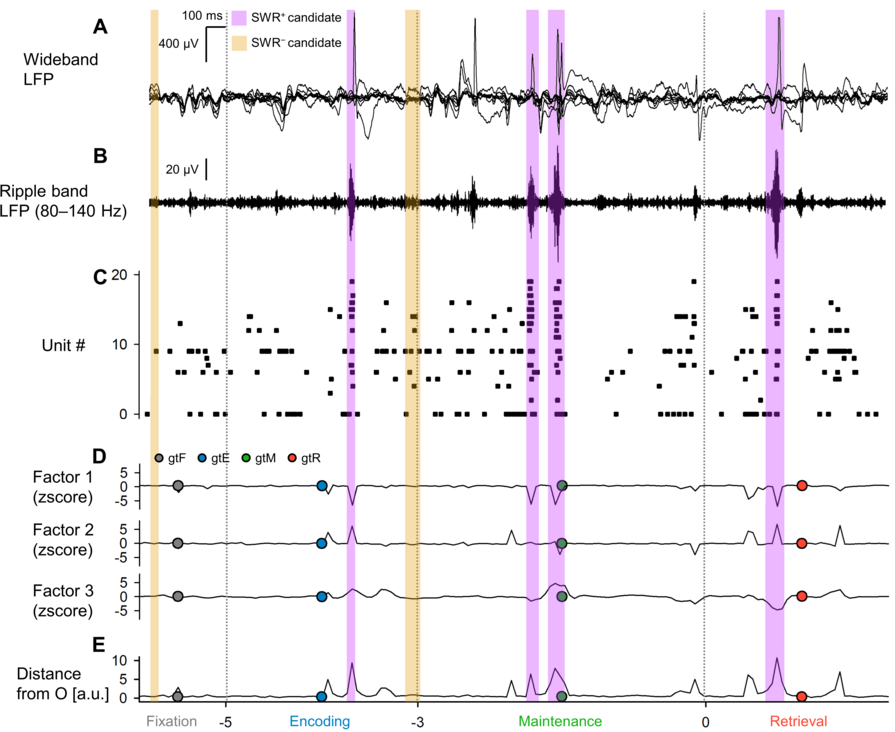
\includegraphics[width=1\textwidth]{./src/figures/.png/Figure_ID_01.png}
        	\caption{\textbf{
Local Field Potentials (LFP), Multiunit Activity, and Neural Trajectories in the Hippocampus During a Modified Sternberg Task
}
\smallskip
\\
\textbf{\textit{A.}} The presented traces illustrate representative wideband LFP intracranial EEG (iEEG) signals, recorded from the left hippocampal head while the subject was performing a modified Sternberg working memory task. This included phases of fixation (1 s, \textit{gray}), encoding (2 s, \textit{blue}), maintenance (3 s, \textit{green}), and retrieval (2 s, \textit{red}). \textbf{\textit{B.}} Subsequently, the corresponding ripple band LFP traces are delineated. \textbf{\textit{C.}} The raster plot represents multiunit spikes drawn from the LFP traces, sorted by a reliable spike-sorting algorithm \cite{niediek_reliable_2016}. \textbf{\textit{D.}} Following that, we portray the neural trajectories, which have been computed using GPFA on spike counts per unit within 50-ms bins. Each phase's geometric median is denoted by dot circles. \textbf{\textit{E.}} The distance of the trajectory from the origin $O$ is presented, with \textit{purple} and \textit{yellow} rectangles indicating the timings for SWR$^+$ candidates and SWR$^-$ candidates (acting as controls for SWR$^+$), respectively.
}
% width=1\textwidth
        	\label{fig:01}
        \end{figure*}
        \clearpage
        \begin{figure*}[ht]
            \pdfbookmark[2]{ID 02}{figure_id_02}
        	\centering
            \includegraphics[width=0.5\textwidth]{./src/figures/.png/Figure_ID_02.png}
        	\caption{\textbf{
State-Dependent Trajectories of Hippocampal Neurons
}
\smallskip
\\
\textbf{\textit{A.}} This panel depicts neural trajectories within the first three-dimensional factors derived from Gaussian Process Factor Analysis (GPFA). Smaller dots represent coordinates corresponding to 50-ms neural trajectory bins. Meanwhile, larger dots with \textit{black} borders denote geometric medians for different stages in the Sternberg working memory task, as follows: fixation (\textit{gray}), encoding (\textit{blue}), maintenance (\textit{green}), and retrieval (\textit{red}). \textbf{\textit{B.}} The graph presents the log-likelihood of the GPFA models compared with the number of dimensions used to embed multiunit spikes from the medial temporal lobe (MTL) territories. Specifically, the optimal dimension, as indicated by the elbow method, was found to be three. \textbf{\textit{C.}} This figure illustrates the distance of the neural trajectories from the origin ($O$) for the hippocampus (Hipp.), entorhinal cortex (EC), and amygdala (Amy.), over time following the probe onset. \textbf{\textit{D.}} The panel displays distances of the trajectories from $O$ within the MTL areas. The hippocampus demonstrates the greatest distance, followed by the EC and the Amygdala. \textbf{\textit{E.}} This graph displays the distances between phases of the trajectories within the MTL regions.
Abbreviations:
}
% width=0.5\textwidth
        	\label{fig:02}
        \end{figure*}
        \clearpage
        \begin{figure*}[ht]
            \pdfbookmark[2]{ID 03}{figure_id_03}
        	\centering
            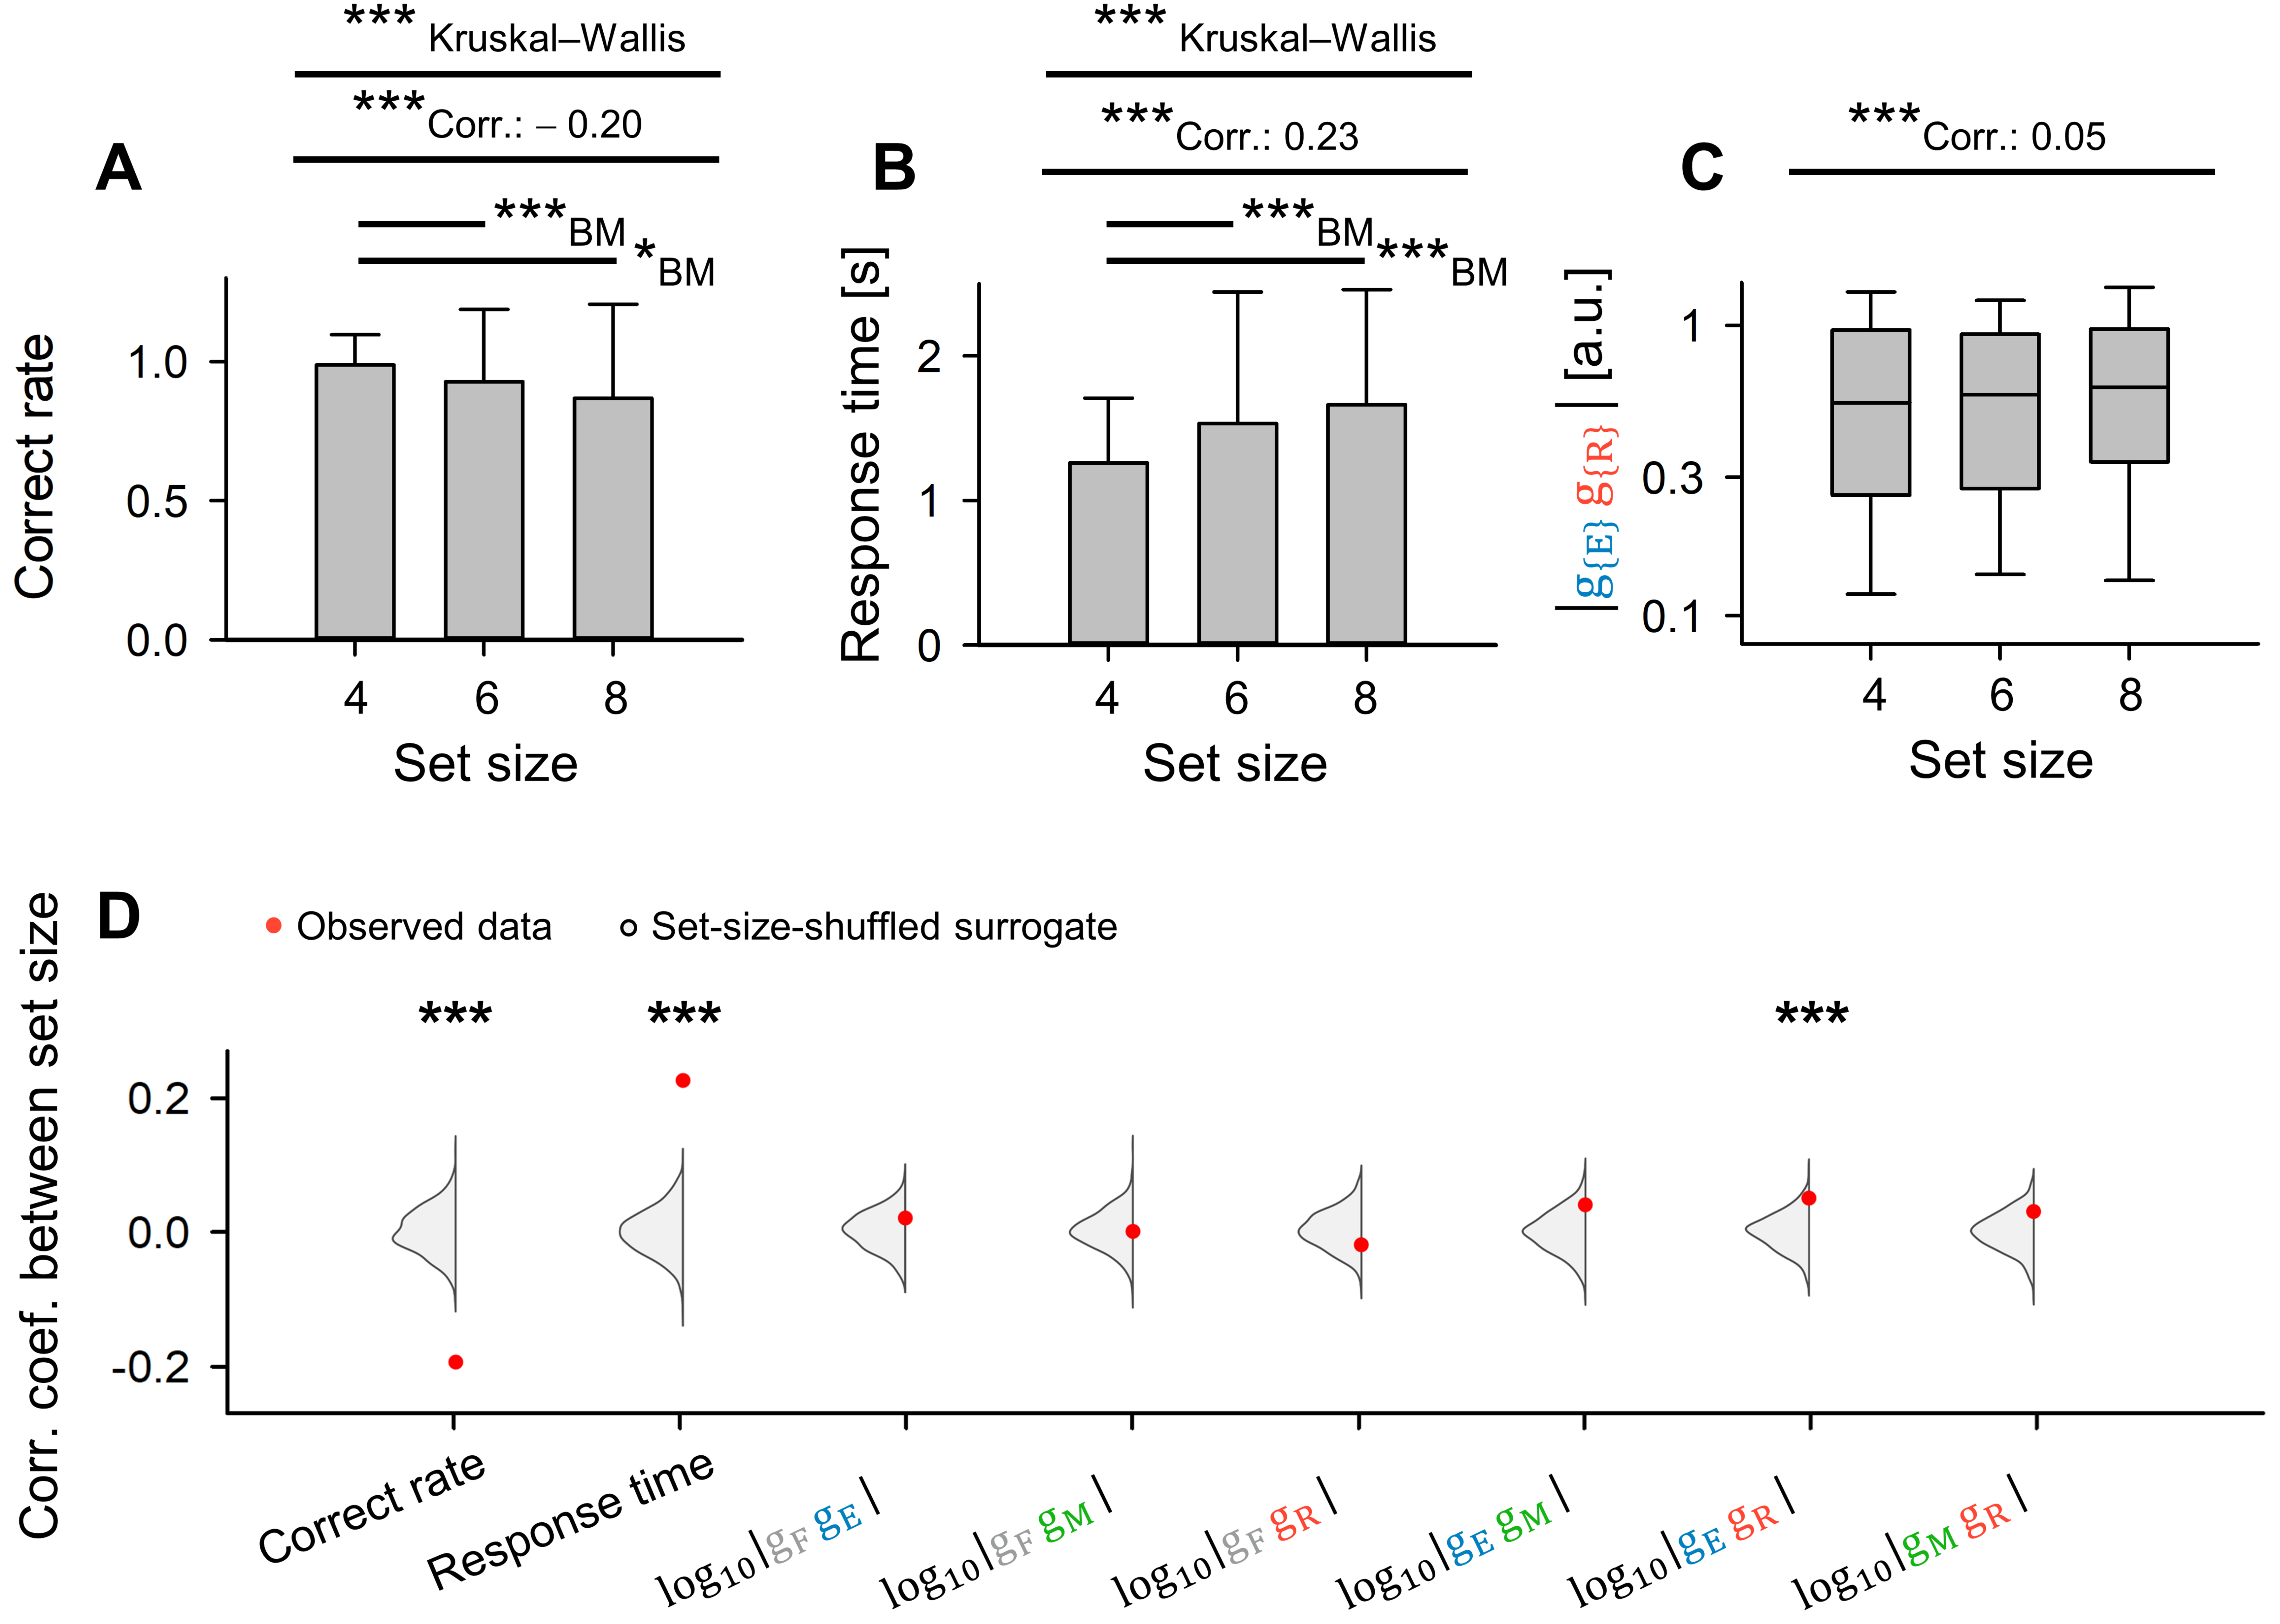
\includegraphics[width=1\textwidth]{./src/figures/.png/Figure_ID_03.png}
        	\caption{\textbf{
Dependency of Trajectory Distance on Memory Load: Encoding and Retrieval States in the Hippocampus.
}
\smallskip
\\
\textbf{\textit{A.}} Illustrates the relationship between set size (the number of letters that require encoding) and the correct rate in the working memory task (coefficient = $-0.20$, ***\textit{p} $<$ 0.001). \textbf{\textit{B.}} Showcases the correlation between set size and response time (coefficient = 0.23, ***\textit{p} $<$ 0.001). \textbf{\textit{C.}} Depicts the influence of set size on the inter-phase distances between the encoding and retrieval phases ($\lVert \mathrm{g_{E}g_{R}} \rVert$) (correlation coefficient = 0.05). \textbf{\textit{D.}} \textit{Red} dots represent experimental observations of correlations between set size and the ensuing parameters: correct rate, response time, $\log_{10}{\lVert \mathrm{g_{F}g_{E}} \rVert}$, $\log_{10}{\lVert \mathrm{g_{F}g_{M}} \rVert}$, $\log_{10}{\lVert \mathrm{g_{F}g_{R}} \rVert}$, $\log_{10}{\lVert \mathrm{g_{E}g_{M}} \rVert}$, $\log_{10}{\lVert \mathrm{g_{E}g_{R}} \rVert}$, and $\log_{10}{\lVert \mathrm{g_{M}g_{R}} \rVert}$. The \textit{gray} kernel density plot demonstrates the corresponding set-size-shuffled surrogate (\textit{n} = 1,000) (***\textit{p}s $<$ 0.001).
}
% width=1\textwidth
        	\label{fig:03}
        \end{figure*}
        \clearpage
        \begin{figure*}[ht]
            \pdfbookmark[2]{ID 04}{figure_id_04}
        	\centering
            \includegraphics[width=1\textwidth]{./src/figures/.png/Figure_ID_04.png}
        	\caption{\textbf{
Detection of SWRs in Prospective CA1 Regions
}
\smallskip
\\
\textbf{\textit{A.}} A two-dimensional UMAP (Uniform Manifold Approximation and Projection) \cite{mcinnes_umap_2018} projection that utilizes multiunit spikes is presented during SWR$^+$ candidates (\textit{purple}) and SWR$^-$ candidates (\textit{yellow}). \textbf{\textit{B.}} A cumulative density plot displaying silhouette scores, indicative of the UMAP clustering quality, is provided for hippocampal regions (Table~\ref{tab:02} as reference). Hippocampal regions that exhibit silhouette scores greater than 0.60, equivalent to the $75^{th}$ percentile, are identified as probable CA1 regions. SWR$^+$ and SWR$^-$ candidates obtained from these hypothetical CA1 regions are respectively categorized as SWR$^+$ and SWR$^-$ (with \textit{n}s = 1,170). \textbf{\textit{C.}} The same distributions of durations are presented for both SWR$^+$ (\textit{purple}) and SWR$^-$ (\textit{yellow}) due to their similar natures (93.0 [65.4] ms, expressed as median [IQR]). \textbf{\textit{D.}} An illustration of the SWR incidence for both the SWR$^+$ (\textit{purple}) and SWR$^-$ (\textit{yellow}) relative to the probe's timing is conveyed as a mean with a 95\% confidence interval. However, given that the intervals may not be noticeable due to their slender range, it should be highlighted that a significant rise in SWR incidence was discovered during the beginning 400 ms of the retrieval phase (0.421 [Hz], *\textit{p} $<$ 0.05, verified by a bootstrap test). \textbf{\textit{E.}} The distributions of ripple band peak amplitudes for SWR$^-$ (\textit{yellow}; 2.37 [0.33] SD of baseline, median [IQR]) and SWR$^+$ (\textit{purple}; 3.05 [0.85] SD of baseline, median [IQR]) are outlined (***\textit{p} $<$ 0.001, confirmed by the Brunner--Munzel test).
}
% width=1\textwidth
        	\label{fig:04}
        \end{figure*}
        \clearpage
        \begin{figure*}[ht]
            \pdfbookmark[2]{ID 05}{figure_id_05}
        	\centering
            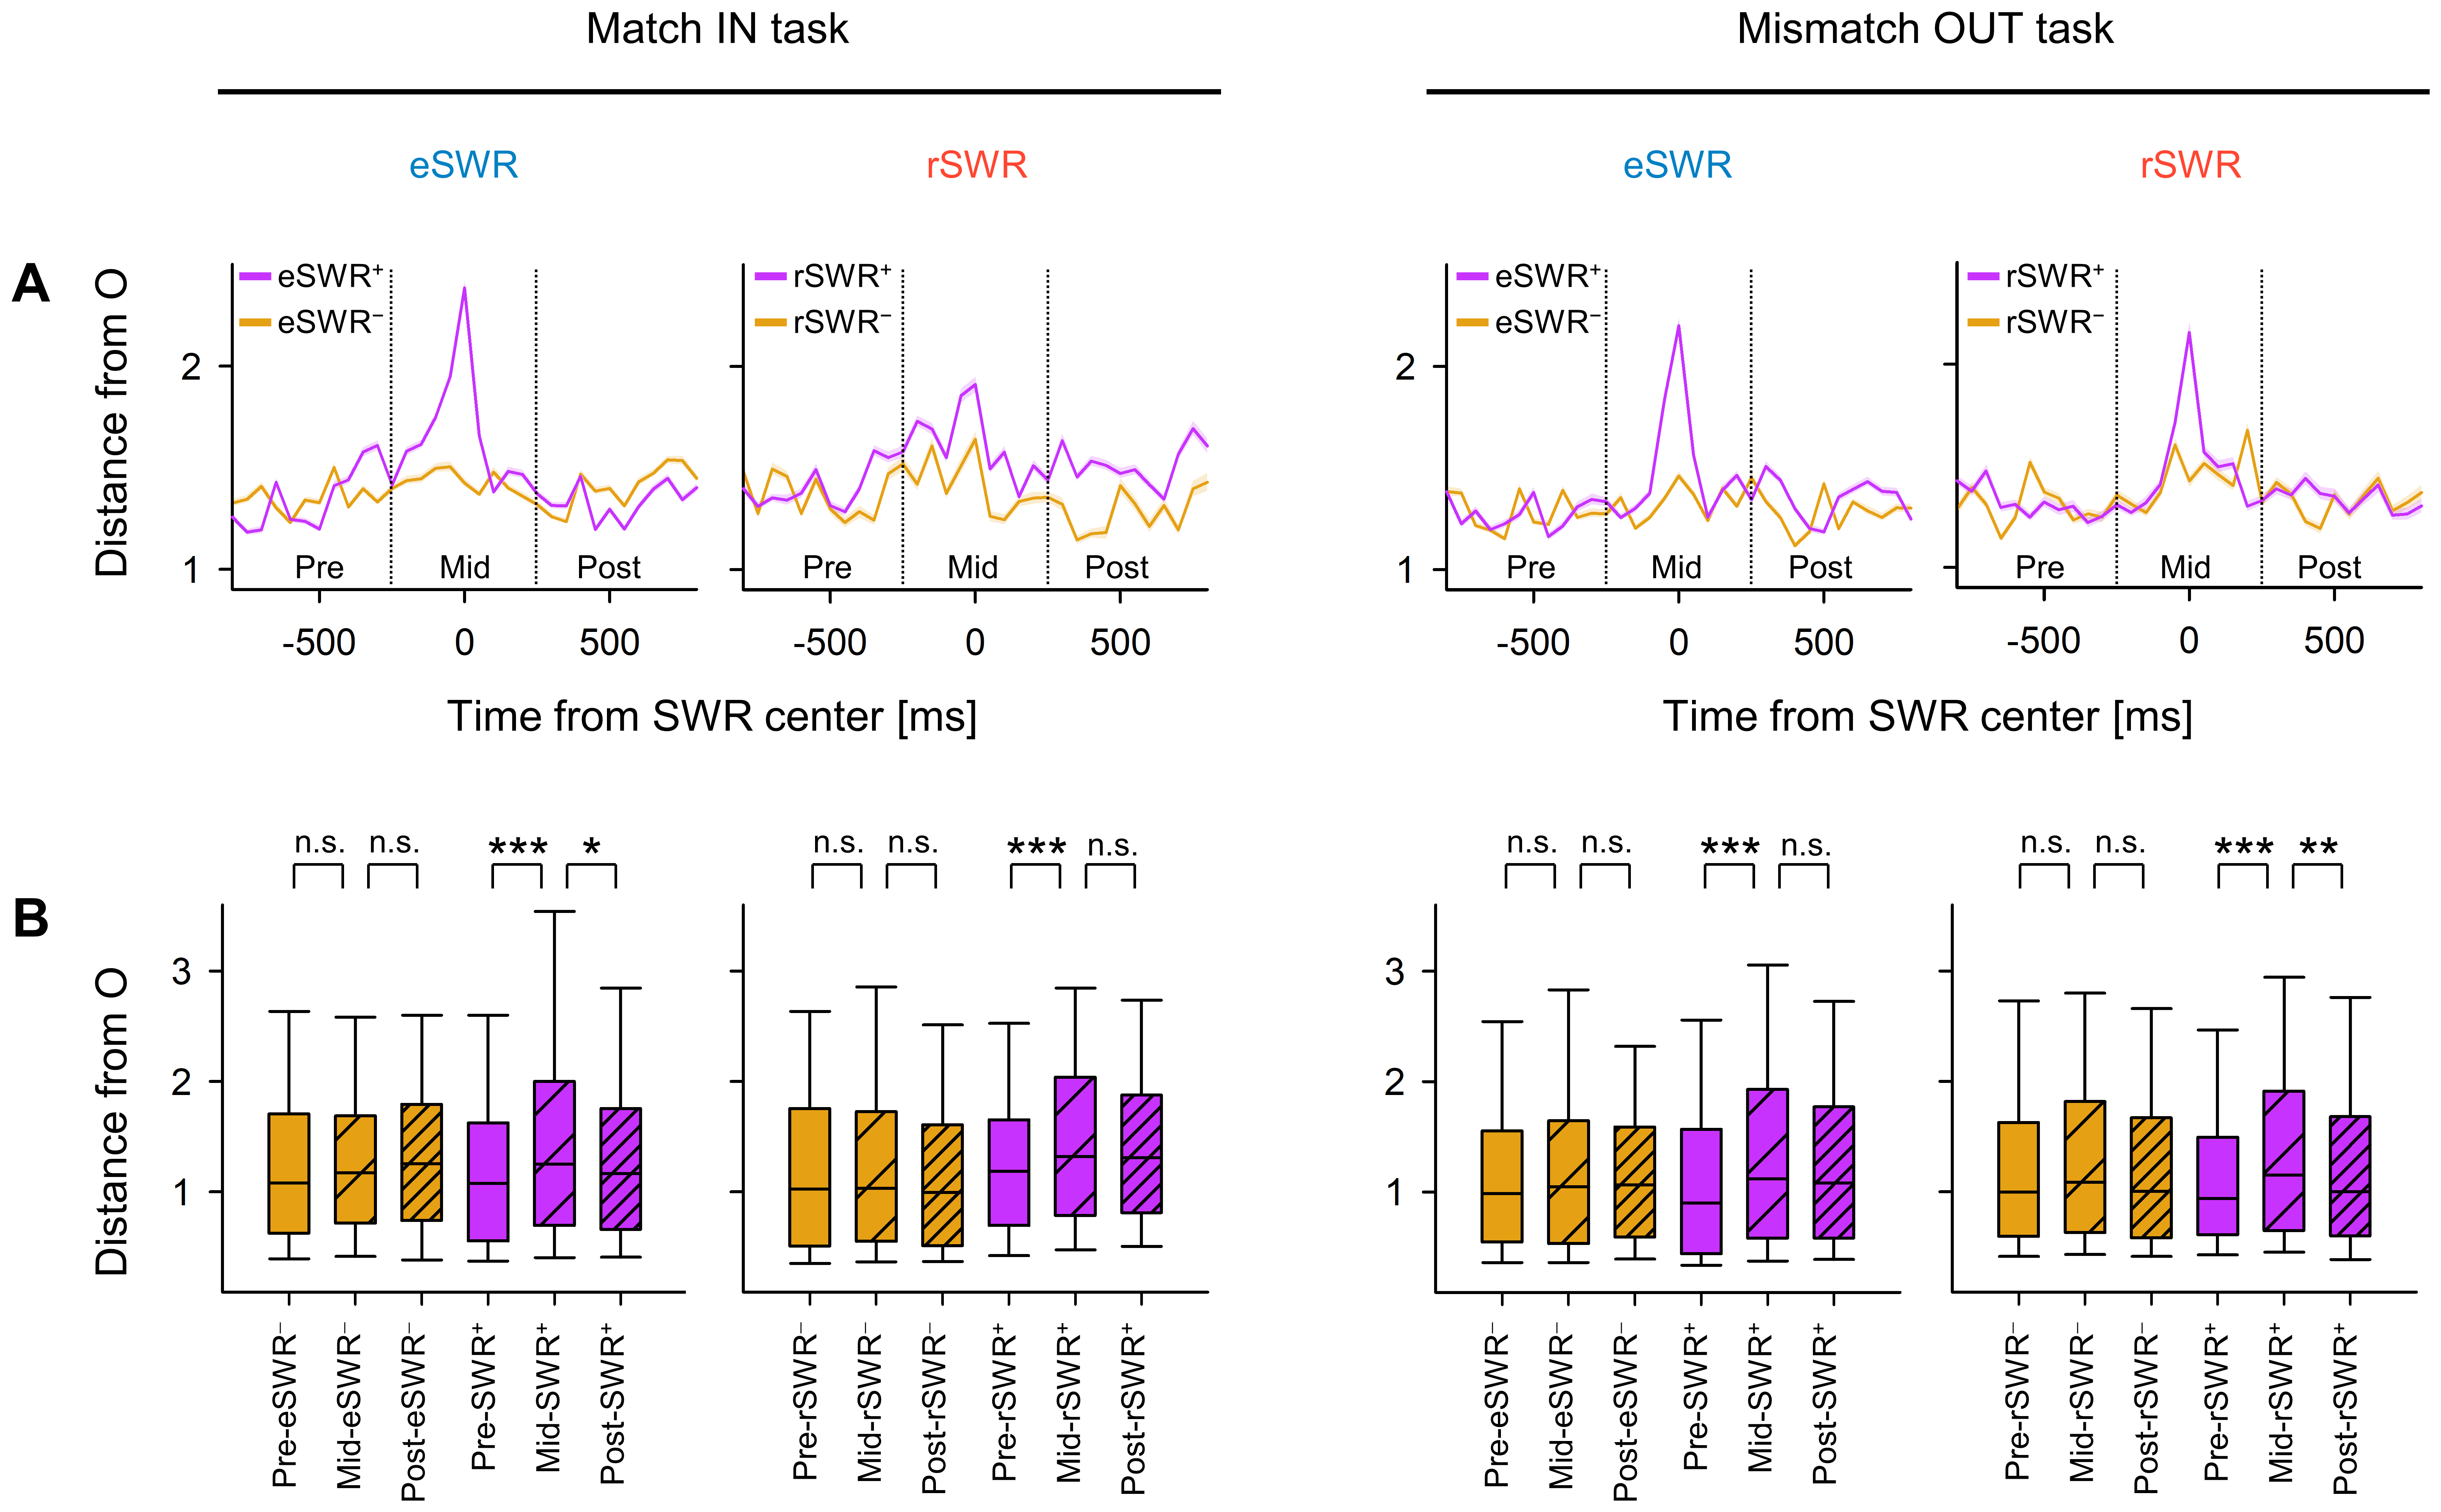
\includegraphics[width=1\textwidth]{./src/figures/.png/Figure_ID_05.png}
        	\caption{\textbf{
Transient Changes in Neural Trajectory During SWR Events
}
\smallskip
\\
\textbf{\textit{A.}} Depicted is the distance from the origin ($O$) of the peri-sharp-wave-ripple (SWR) trajectory, calculated as the mean \textpm 95\% confidence interval. The intervals might not be noticeable due to their narrow magnitudes. \textbf{\textit{B.}} Illustrated is the distance from the origin ($O$) during the pre-, mid-, and post-SWR phases (*\textit{p} $<$ 0.05, **\textit{p} $<$ 0.01, ***\textit{p} $<$ 0.001; evaluated using the Brunner--Munzel test). Abbreviations: SWR, sharp-wave ripple events; eSWR, SWR within the encoding phase; rSWR, SWR during retrieval phase; SWR$^+$, positive SWR event; SWR$^-$, control events for SWR$^+$; pre-, mid-, or post-SWR refer to the time intervals from $-800$ to $-250$ ms, from $-250$ to $+250$ ms, or from $+250$ to $+800$ ms, all in relation to the central point of the SWR.
}
% width=1\textwidth
        	\label{fig:05}
        \end{figure*}
        \clearpage
        \begin{figure*}[ht]
            \pdfbookmark[2]{ID 06}{figure_id_06}
        	\centering
            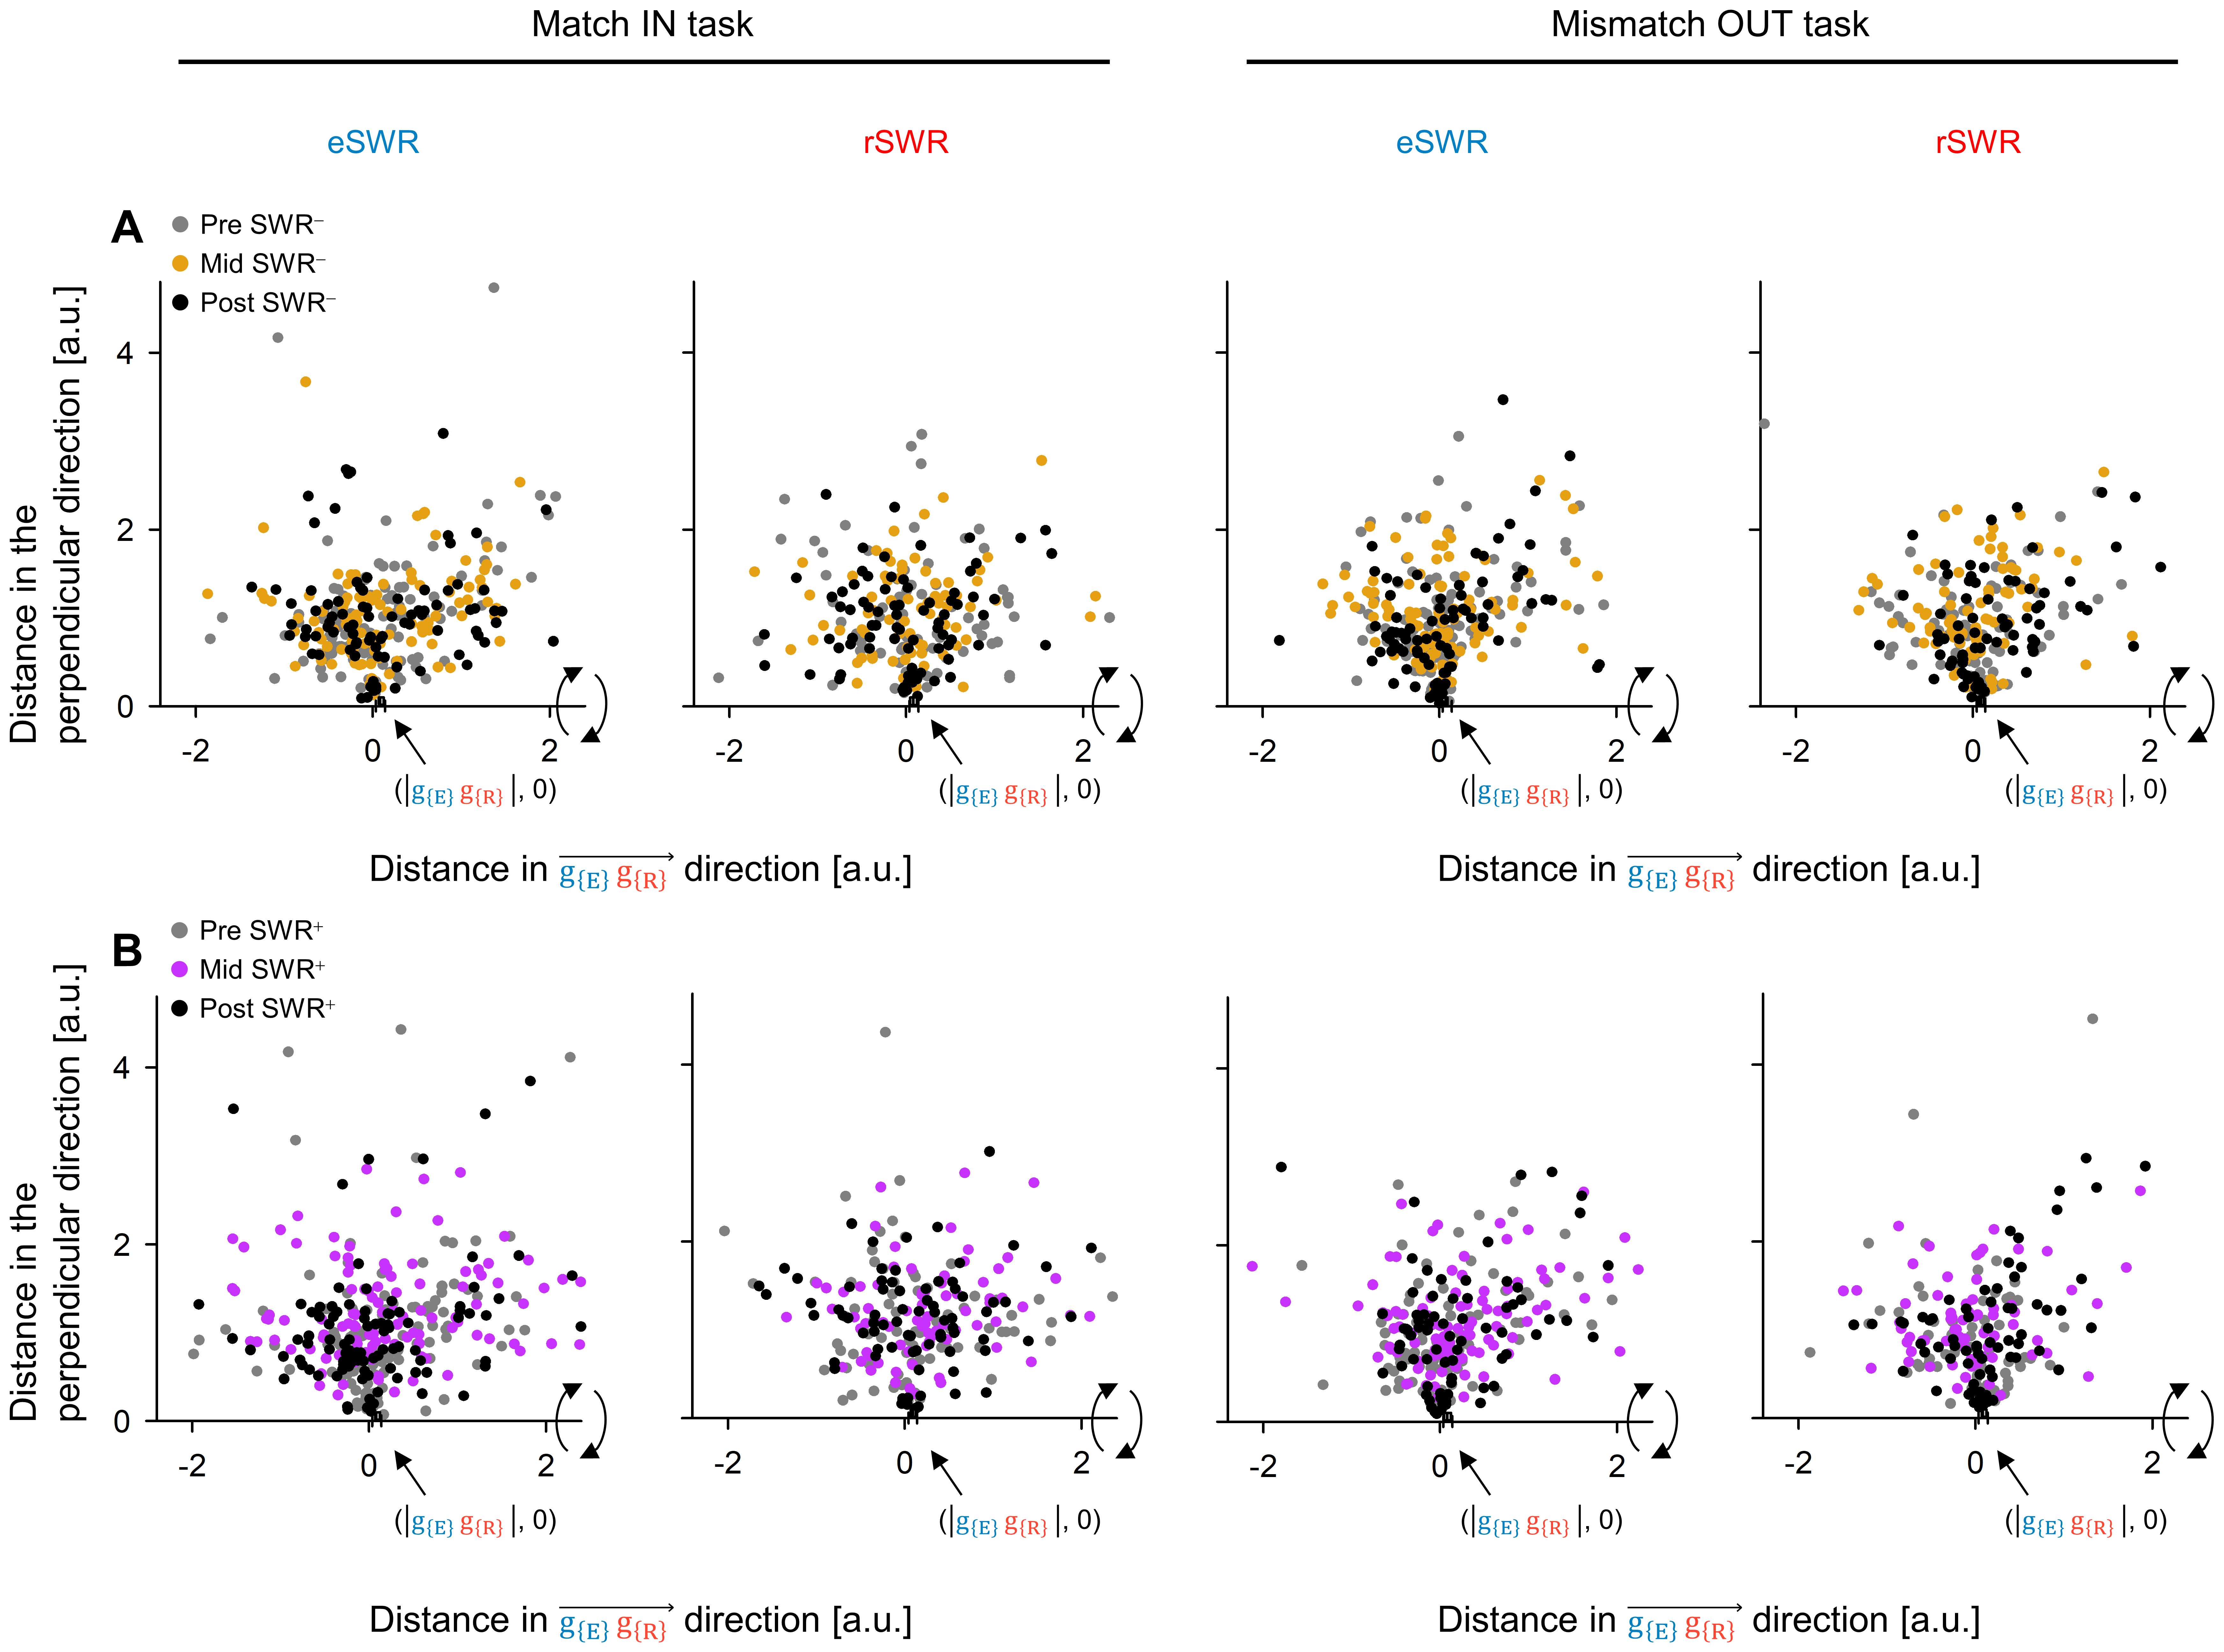
\includegraphics[width=1\textwidth]{./src/figures/.png/Figure_ID_06.png}
        	\caption{\textbf{
Visualizing Neural Trajectories during SWR in Two-Dimensional Spaces}
\smallskip
\\
The figures depict hippocampal neural trajectories during SWR, projected onto two-dimensional spaces. \textbf{\textit{A.}} Displays hippocampal neural trajectories before (pre), during (mid), and after (post) SWR$^-$, denoted in \textit{gray}, \textit{yellow}, and \textit{black}, respectively. \textbf{\textit{B.}} Shows the corresponding trajectories for SWR$^+$. The magnitude of $\lVert \mathrm{g_{E}g_{R}} \rVert$ varied across sessions. The following projection method was employed: Firstly, a linear transformation positioned $\mathrm{g_{E}}$ at origin $O$ (0,0), and $\mathrm{g_{R}}$ at ($\lVert \mathrm{g_{E}g_{R}} \rVert$, 0). The point cloud was then rotated around the $\mathrm{g_{E}g_{R}}$ axis (identical to the x-axis) to fit into the two-dimensional spaces. Consequently, within these two-dimensional spaces, the distances from $O$ and the angles remained consistent with the original properties of the $\mathrm{g_{E}g_{R}}$ axis in the three-dimensional spaces. Abbreviations: SWR refers to sharp-wave ripple events; eSWR represents SWR during the encoding phase; rSWR denotes SWR during retrieval phase; SWR$^+$ indicates an occurrence of SWR event; SWR$^-$ refers to control events for SWR$^+$; pre-SWR, mid-SWR, or post-SWR refer to time intervals from $-800$ to $-250$ ms, from $-250$ to $+250$ ms, or from $+250$ to $+800$ ms from the center of SWR, respectively.}
% width=1\textwidth
        	\label{fig:06}
        \end{figure*}
        \clearpage
        \begin{figure*}[ht]
            \pdfbookmark[2]{ID 07}{figure_id_07}
        	\centering
            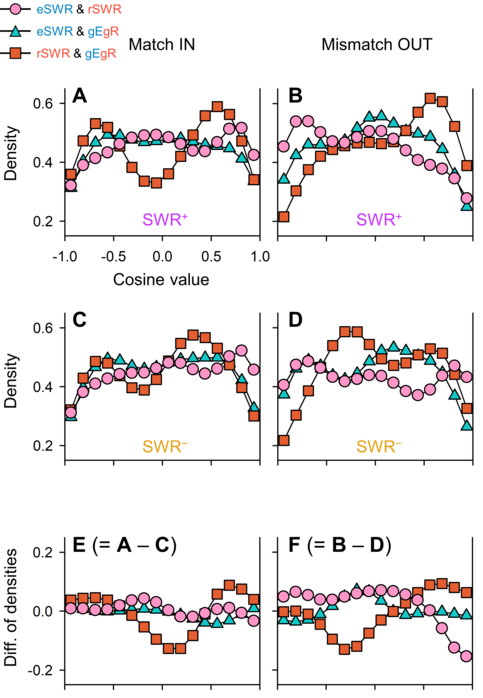
\includegraphics[width=0.5\textwidth]{./src/figures/.png/Figure_ID_07.png}
        	\caption{\textbf{
Neural Trajectory Directions during SWRs: Encoding and Retrieval States
}
\smallskip
\\
\textbf{\textit{A--B}} Kernel density estimation (KDE) distributions of $\protect\overrightarrow{{\mathrm{eSWR^+}}} \cdot \protect\overrightarrow{{\mathrm{rSWR^+}}}$ (\textit{pink circles}), $\protect\overrightarrow{{\mathrm{eSWR^+}}} \cdot \protect\overrightarrow{{\mathrm{g_{E}g_{R}}}}$ (\textit{blue triangles}), and $\protect\overrightarrow{{\mathrm{rSWR^+}}} \cdot \protect\overrightarrow{{\mathrm{g_{E}g_{R}}}}$ (\textit{red rectangles}) are shown for Match IN (\textit{A}) and Mismatch OUT tasks (\textit{B}). \textbf{\textit{C--D}} Display the corresponding distributions of $\mathrm{SWR^-}$ replacing those of $\mathrm{SWR^+}$ in \textit{A} and \textit{B}. \textbf{\textit{E--F}} Illustrate the discrepancies in the distributions of $\mathrm{SWR^+}$ and $\mathrm{SWR^-}$, highlighting the SWR components (\textit{E} = \textit{C} $-$ \textit{A}; \textit{F} = \textit{D} $-$ \textit{B}). Observe the biphasic distributions of $\protect\overrightarrow{{\mathrm{rSWR^-}}} \cdot \protect\overrightarrow{{\mathrm{g_{E}g_{R}}}}$, indicating fluctuations between the encoding and retrieval states throughout the Sternberg task. Additionally, contrasting directionality between $\protect\overrightarrow{{\mathrm{eSWR^+}}}$ and $\protect\overrightarrow{{\mathrm{rSWR^+}}}$ was noticed (\textit{pink circles}) in the Mismatch OUT task, but was absent in the Match IN task (\textbf{\textit{E--F}}). Lastly, transitions from the retrieval to the encoding states were prominent in the SWR components in both the Match IN and Mismatch OUT tasks (\textit{red rectangles} in \textit{E} and \textit{F}).
}
% width=0.5\textwidth
        	\label{fig:07}
        \end{figure*}

%%%%%%%%%%%%%%%%%%%%%%%%%%%%%%%%%%%%%%%%%%%%%%%%%%%%%%%%%%%%%%%%%%%%%%%%%%%%%%%%
%% END
%%%%%%%%%%%%%%%%%%%%%%%%%%%%%%%%%%%%%%%%%%%%%%%%%%%%%%%%%%%%%%%%%%%%%%%%%%%%%%%%

\end{document}
